\subsection{TAOCP 7.1.3 Exercise 203, MMIX MOR instruction and program synthesis by sketching}

Found this exercise in TAOCP 7.1.3 (Bitwise Tricks and Techniques):

% TODO: border
\begin{figure}[H]
\centering
\frame{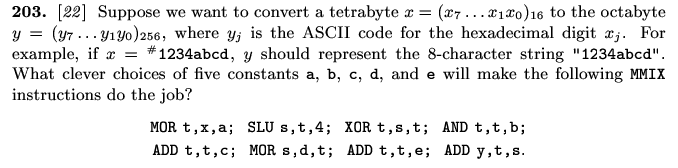
\includegraphics[scale=0.7]{pgm_synth/TAOCP_713_203/203q.png}}
\caption{Screenshot from TAOCP book}
\end{figure}

What is MOR instruction in MMIX?

\begin{figure}[H]
\centering
\frame{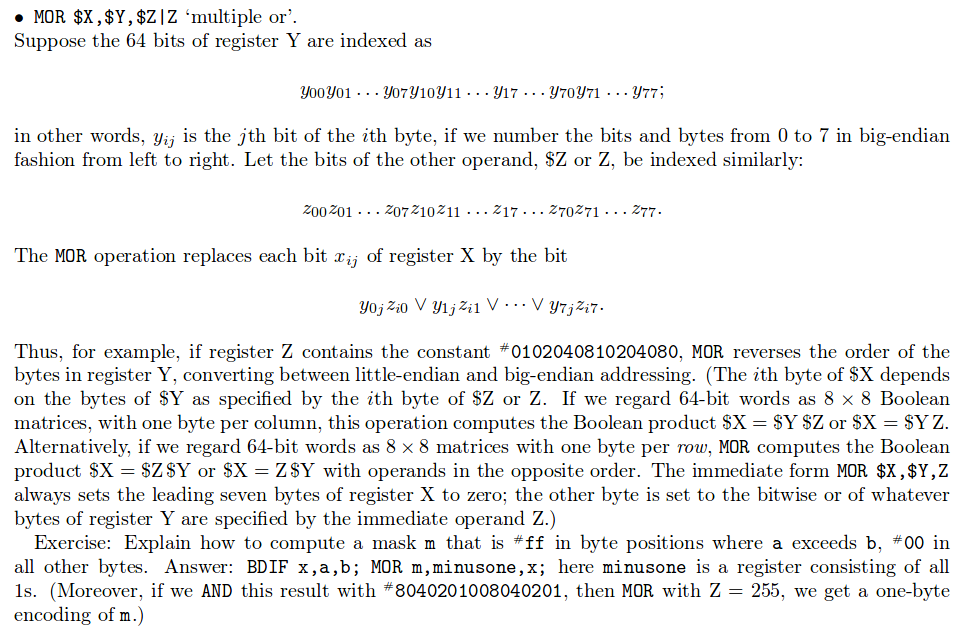
\includegraphics[scale=0.55]{pgm_synth/TAOCP_713_203/MOR.png}}
\caption{Screenshot from the MMIX book}
\end{figure}

( \url{http://mmix.cs.hm.edu/doc/mmix-doc.pdf} )

Let's try to solve. We create two functions. First has MOR instructions simulation + the program from TAOCP.
The second is a naive implementation.
Then we add ``forall'' quantifier: for all inputs, both functions must produce the same result.
\textbf{But}, we don't know a/b/c/d/e/f and ask Z3 SMT-solver to

\lstinputlisting[style=custompy]{pgm_synth/TAOCP_713_203/v1.py}

Very slow, it takes several hours on my venerable Intel Quad-Core Xeon E3-1220 3.10GHz but found at least one solution:

\begin{lstlisting}
a,b,c,d,e = 8000400020001 f0f0f0f0f0f0f0f 56d656d616969616 411a00000000 bf3fbf3fff7f8000
\end{lstlisting}

\dots which is correct (I've wrote bruteforce checker, here: \url{https://github.com/DennisYurichev/SAT_SMT_by_example/blob/master/pgm_synth/TAOCP_713_203/check.c}.

D.Knuth's TAOCP also has answers:

\begin{figure}[H]
\centering
\frame{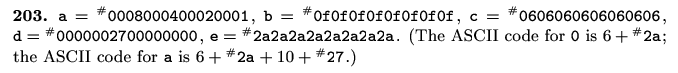
\includegraphics[scale=0.6]{pgm_synth/TAOCP_713_203/203a.png}}
\caption{Screenshot from TAOCP book}
\end{figure}

\dots which are different, but also correct.

What if a==0x0008000400020001 always?
I'm adding a new constraint:

\begin{lstlisting}
s.add(a==0x0008000400020001)
\end{lstlisting}

We've getting many results (much faster, and also correct):

\begin{lstlisting}
...

a,b,c,d,e = 8000400020001 7f0fcf0fcf0f7f0f 1616d6d656561656 8680522903020000 eeeda9aa2e2eee2f
a,b,c,d,e = 8000400020001 7f0fcf0fcf0f6f0f 1616d6d656561656 8680522903020000 eeeda9aa2e2eee2f
a,b,c,d,e = 8000400020001 7f0fcf0fdf0f6f0f 1616d6d656561656 8680522903020000 eeeda9aa2e2eee2f
a,b,c,d,e = 8000400020001 5f0fcf0fdf0f6f0f 1616d6d656561656 8680522903020000 eeeda9aa2e2eee2f

...
\end{lstlisting}

The files: \url{https://github.com/DennisYurichev/SAT_SMT_by_example/tree/master/pgm_synth/TAOCP_713_203}.

